\documentclass[11pt,a4paper]{report}

\usepackage[a4paper, margin=1in]{geometry}
\usepackage{polski}
\usepackage[utf8]{inputenc}
\usepackage{indentfirst}
\usepackage{hyperref}
\usepackage{tikz}
\usepackage{pgf-umlcd}
\usepackage{tikz-among-us}
\usepackage{graphicx}

\graphicspath{ {./images/} }

\def\console #1{\begingroup\fontfamily{qcr}\selectfont#1\endgroup}
\newenvironment{multiconsole}{\begingroup\fontfamily{qcr}\selectfont}{\endgroup}



\title{\Huge JavaGridGraph - Dokumentacja}
\author{Skoczek Mateusz, Jędrzejewski Sebastian}
\date{\today}



\begin{document}
    \maketitle
        




    \begin{abstract}
        Dokument zawiera specyfikację funkcjonalną i implementacyjną dotyczącą projektu \textsl{JavaGridGraph} oraz opis testów programu.
    \end{abstract}





    \tableofcontents
    \thispagestyle{empty}





    \newpage
    \chapter{Specyfikacja funkcjonalna}




    \newpage
    \section{Cel projektu}

    Program \textbf{JavaGridGraph} ma na celu umożliwiać wykonanie dwóch podstawowych zadań

    \begin{itemize}
        \item wygenerowanie grafu siatkowego o podanych paramentrach
        \item sprawdzenie wybranych parametrów dowolnego grafu siatkowego
    \end{itemize}

    Program posiada interfejs graficzny. Grafy są przedstawiane w plikach w postaci listy sąsiedztwa.




    \newpage
    \section{Opis funkcji}

    Program oferuje dwie główne funkcje: generowanie grafu oraz sprawdzanie grafu.

    \vspace{4em}

    Program pozwala wygenerować graf o:
    
    \begin{itemize}
        \item określonej wysokości (ilości wierszy)
        \item określonej szerokości (ilości kolumn)
        \item określonej minimalnej i maksymalnej wadze krawędzi
        \item określonej minimalnej i maksymalnej ilości krawędzi wychodzących z pojedyńczego wierzchołka (dla grafu skierowanego)
        \item określonej minimalnej i maksymalnej ilości krawędzi wchodzących do pojedyńczego wierzchołka (dla grafu skierowanego)
        \item określonej minimalnej i maksymalnej ilości "sąsiadów" pojedyńczego wierzchołka (dla grafu nieskierowanego)
        \item niestandardowym ziarnie generatora liczb losowych
    \end{itemize}

    Program umożliwia zapis wygenerowanego grafu do pliku oraz/lub wczytanie grafu do sprawdzenia.
    
    \vspace{4em}

    W ramach funkcji sprawdzania grafu, program pozwala na sprawdzenie następujących parametrów wczytanego grafu:

    \begin{itemize}
        \item spójność grafu
        \item najkrótsze ścieżki od wybranego wierzchołka $A$ do wybranych wierzchołków $B_n$
    \end{itemize}




    \newpage
    \section{Opis interfejsu programu}

    \subsection{Okno główne - widok startowy}

    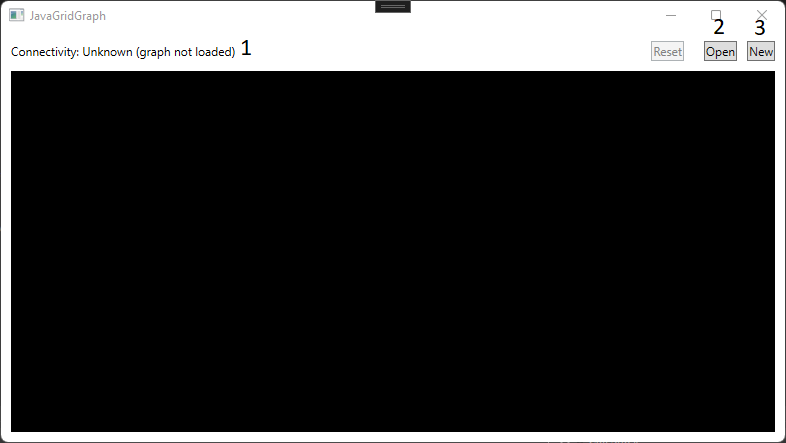
\includegraphics[width=\textwidth]{view1.png}

    \begin{enumerate}
        \item Wynik sprawdzenia spójności grafu. W przypadku gdy graf nie został wczytany, zostanie pokazana informacja o tym że graf nie został wczytany.
        \item Przycisk "Open" otwiera systemowe okno wyboru pliku w celu wybrania pliku zawierającego graf.
        \item Przycisk "New" otwiera okno generowania grafu. Więcej informacji w punkcie "Okno generowania grafu".
    \end{enumerate}

    \subsection{Okno generowania grafu}

    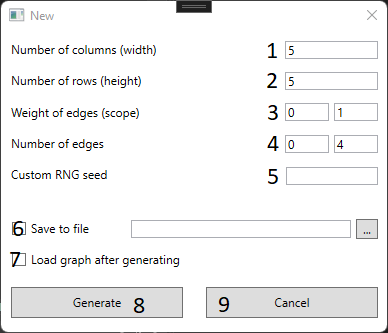
\includegraphics[width=\textwidth]{view2.png}

    \begin{enumerate}
        \item Liczba kolumn (szerokość) grafu. Pole nie może być puste.
        \item Liczba wierszy (wysokość) grafu. Pole nie może być puste.
        \item Waga krawędzi. Wartość w pierwszym polu (min, domyślnie 0) musi być mniejsza bądź równa wartości w drugim polu (max, domyślnie 1).
        \item Wybór między generowaniem grafu skierowanego (directed), generowaniem grafu nieskierowanego (not directed).
        \item Liczba krawędzi wychodzących z pojedyńczego wierzchołka. Wartość w pierwszym polu (min, domyślnie 0) musi być mniejsza bądź równa wartości w drugim polu (max, domyślnie 4). [Tylko gdy zaznaczone generowanie grafu skierowanego]\footnote{Program będzie dążył do utworzenia co najmniej minimalnej liczby krawędzi (połączeń do sąsiadów), ale nie może tego zagwarantować. Nie jest możliwe wygenerowanie więcej niż 2 krawędzi dla wierzchołków w narożnikach oraz więcej niż 3 dla wierzchołków bocznych. Nie jest możliwe także utworzenie krawędzi, jeżeli wszystkie wierzchołki wokół osiągnęły już swoją nominalną (wylosowaną z podanego przedziału) liczbę krawędzi.}
        \item Liczba krawędzi wchodzących do pojedyńczego wierzchołka. Wartość w pierwszym polu (min, domyślnie 0) musi być mniejsza bądź równa wartości w drugim polu (max, domyślnie 4). [Tylko gdy zaznaczone generowanie grafu skierowanego]\footnotemark[\value{footnote}]
        \item Liczba sąsiadów pojedyńczego wierzchołka. Wartość w pierwszym polu (min, domyślnie 0) musi być mniejsza bądź równa wartości w drugim polu (max, domyślnie 4). [Tylko gdy zaznaczone generowanie grafu nieskierowanego]\footnotemark[\value{footnote}]
        \item Niestandardowe ziarno generatora liczb losowych.
        \item Zaznaczenie tego pola spowoduje zapisanie grafu w pliku wybranym w systemowym oknie zapisu pliku, które wyświetli się po naciśnięciu przycisku "Generate".
        \item Zaznaczenie tego pola spowoduje wczytanie grafu do programu zaraz po jego wygenerowaniu.
        \item Kliknięcie przycisku spowoduje wygenerowanie grafu o podanych parametrach.
    \end{enumerate}

    \subsection{Okno główne - po wczytaniu grafu}

    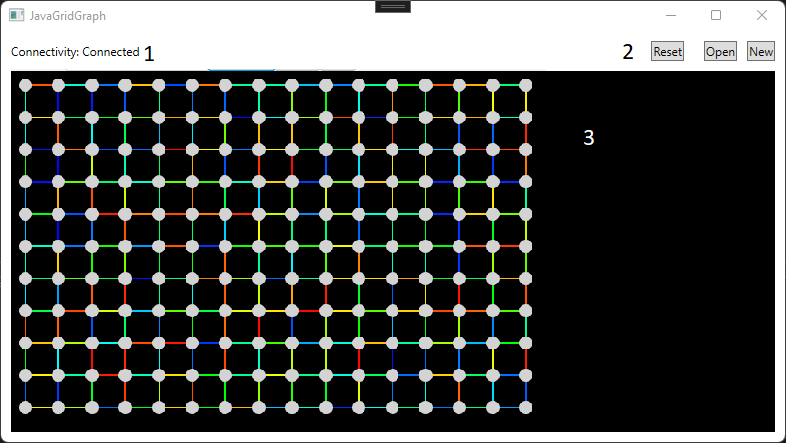
\includegraphics[width=\textwidth]{view3.png}

    \begin{enumerate}
        \item Wynik sprawdzenia spójności grafu. "Connected" - spójny, "Unconnected" - niespójny.
        \item Kliknięcie przycisku spowoduje odznaczenie wszystkich zaznaczonych wierzchołków na grafie.
        \item Pole w którym wyświetlany jest graf. Aby znaleźć najkrótsze ścieżki musimy wybrać wierzchołek $A$ lewym przyciskiem myszy (zostanie zaznaczony na czerwono) oraz wierzchołki $B_n$ prawym przyciskiem myszy (zostaną zaznaczone na zielono). Po wybraniu wierzchołka $A$ oraz przynajmniej jednego wierzchołka $B$ zostanie narysowana najkrótsza ścieżka od wierzchołka $A$ do wierzchołka $B_n$.
    \end{enumerate}




    \newpage
    \section{Format danych wejściowych i wyjściowych}
    Dane wejściowe i wyjściowe przechowują graf w postaci listy sąsiedztwa. W pierwszej linijce znajdują się dwie liczby, które oznaczają odpowiednio liczbę kolumn i wierszy danego grafu. Każda następna linijka reprezentuje jeden wierzchołek, przy czym wierzchołki numerujemy od 0 od lewej do prawej. Zatem druga linijka w pliku zawiera numery wierzchołków, z którymi połączony jest wierzchołek numer 0, kolejna dotyczy wierzchołka numer 1 itd. Przy każdym numerze wierzchołka po dwukropku podana jest waga krawędzi pomiędzy tymi dwoma wierzchołkami.

    \vspace{1em}

    \noindent
    \textbf{Przykład:}

    \begin{multiconsole}
        2 2

        \hspace*{2em}1 :0.54  2 :0.78

        \hspace*{2em}0 :0.54  3 :0.12

        \hspace*{2em}0 :0.78  3 :0.89

        \hspace*{2em}1 :0.12  2 :0.89
    \end{multiconsole}

    Powyżej przedstawiona jest przykładowa zawartość pliku przechowującego graf. W pierwszej linijce można odczytać, że jest to graf o dwóch kolumnach i dwóch wierszach. W drugiej linijce przedstawiona jest informacja o tym, że wierzchołek numer 0 połączony jest z wierzchołkiem numer 1, a krawędź ta ma wagę 0.54. Istnieje również krawędź pomiędzy wierzchołkiem 0 a 2 o wadze 0.78. W trzeciej linijce znajdują się numery wierzchołków połączonych z wierzchołkiem numer 1 wraz z wagami itd.





    \newpage
    \chapter{Specyfikacja implementacyjna}

    \newpage
    \section{Diagram klas}
    \begin{center}
        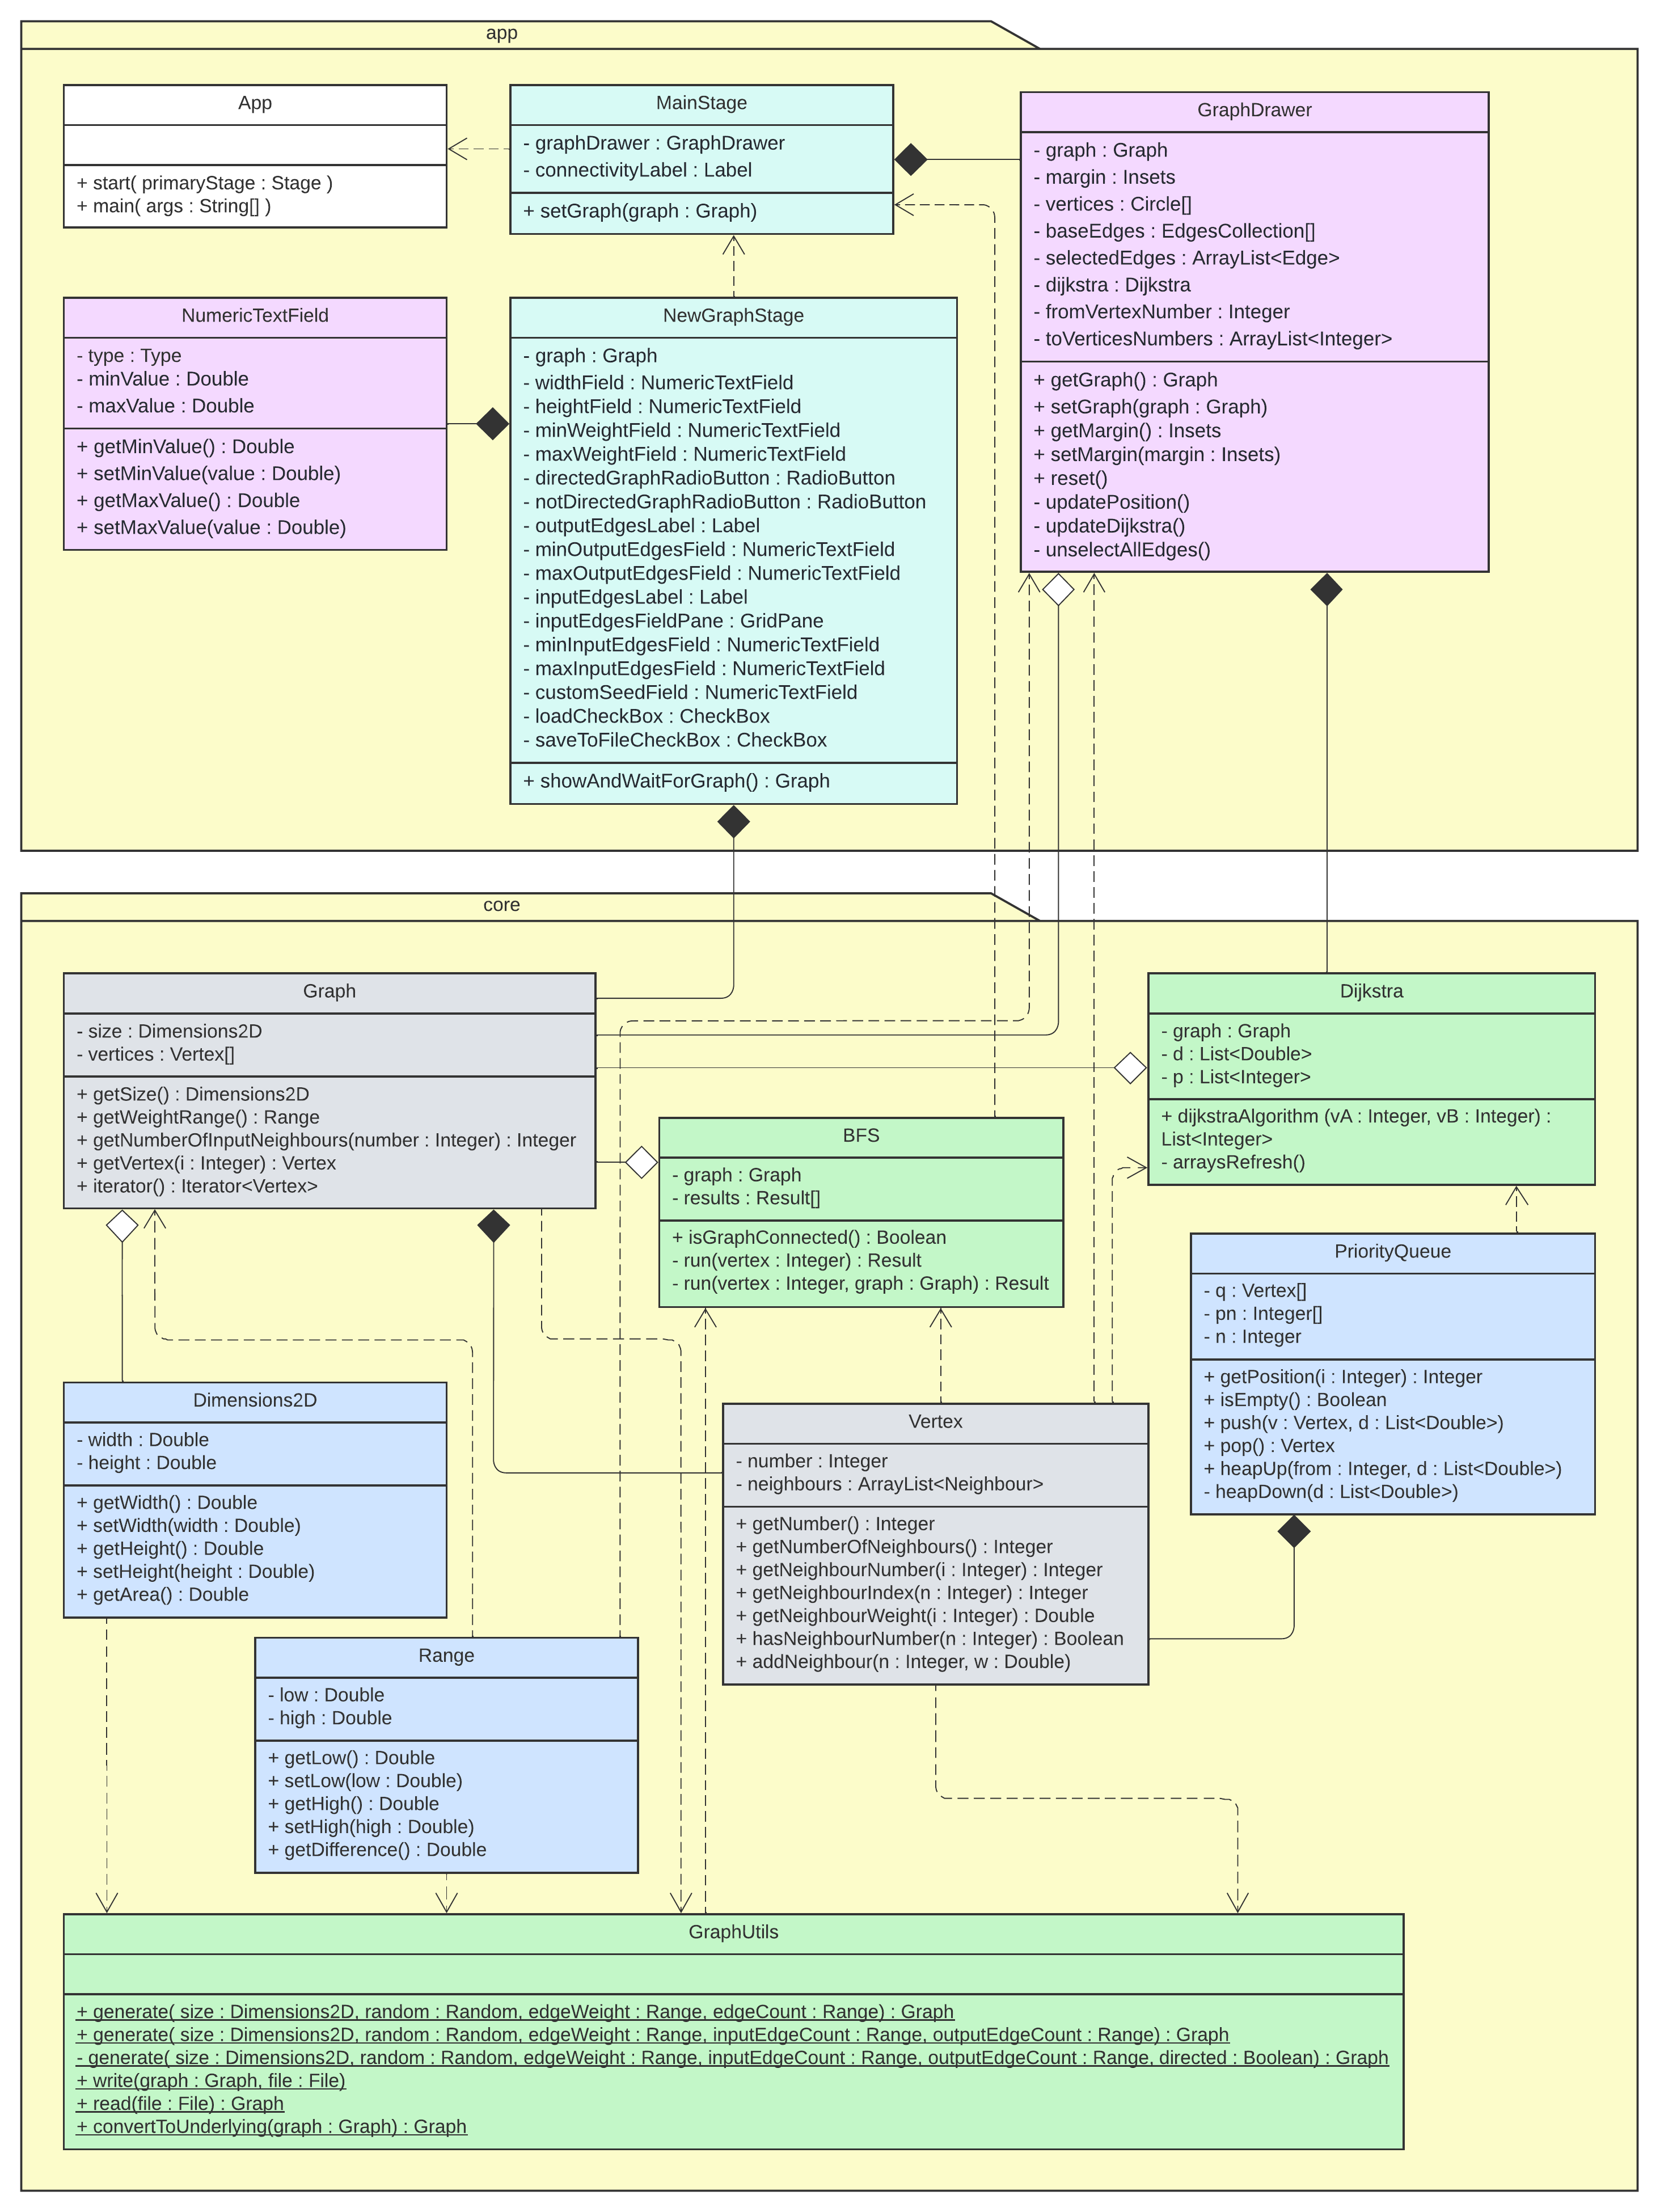
\includegraphics[width=\textwidth]{uml.png}
    \end{center}

    \newpage
    \section{Interfejs (Pakiet App)}

    Interfejs aplikacji został stworzony przy wykorzystaniu biblioteki JavaFX. Pakiet \textbf{App} składa się z dwóch podpakietów:

    \begin{itemize}
        \item \textbf{Controls} zawierającym niestandardowe kontrolki
        \item \textbf{Stages} zawierającym widoki aplikacji
    \end{itemize}

    \newpage
    \subsection{App}

\end{document}